\documentclass{minimal}
\usepackage[T1]{fontenc}
\usepackage{newtxtext}
\usepackage{newtxmath}
\usepackage{xcolor}
\usepackage{tikz}
\usetikzlibrary{arrows.meta,calc,positioning}

\pdfpagewidth=1000pt
\pdfpageheight=360pt
\setlength{\paperwidth}{1000pt}
\setlength{\paperheight}{360pt}
\setlength{\textwidth}{1000pt}
\setlength{\textheight}{360pt}
\setlength{\oddsidemargin}{-72pt}
\setlength{\topmargin}{-72pt}
\setlength{\headheight}{0pt}
\setlength{\headsep}{0pt}
\setlength{\footskip}{0pt}
\setlength{\parindent}{0pt}
\pagestyle{empty}

\begin{document}
\begin{tikzpicture}[
  x=1pt,y=1pt,
  font=\rmfamily,
  line cap=round,
  line join=round
]
\definecolor{tsink}{HTML}{1F2933}
\definecolor{tsmuted}{HTML}{59636E}
\definecolor{tspaper}{HTML}{FFFFFF}
\definecolor{tspanel}{HTML}{F7F9FA}
\definecolor{tsblue}{HTML}{315F80}
\definecolor{tsbluefill}{HTML}{EAF1F5}
\definecolor{tsgreen}{HTML}{2F6B58}
\definecolor{tsgreenfill}{HTML}{E7F2ED}
\definecolor{tspurple}{HTML}{62578A}
\definecolor{tspurplefill}{HTML}{EEEAF5}
\definecolor{tsorange}{HTML}{A85B1A}
\definecolor{tsorangefill}{HTML}{FBF0E4}
\definecolor{tsgrayfill}{HTML}{F0F2F3}

\tikzset{
  inference/.style={
    -{Latex[length=9pt,width=6pt]},
    draw=tsink,
    line width=2.2pt
  },
  training/.style={
    -{Latex[length=8pt,width=5pt]},
    draw=tsorange,
    densely dashed,
    line width=1.9pt,
    preaction={draw=tspaper,line width=5pt}
  },
  query/.style={
    -{Latex[length=7pt,width=5pt]},
    draw=tsmuted,
    densely dotted,
    line width=1.6pt
  },
  module/.style={
    rounded corners=8pt,
    draw=tsink,
    line width=1.55pt,
    fill=tspaper,
    align=center,
    minimum height=48pt,
    inner sep=7pt
  },
  historybox/.style={module,draw=tsblue,fill=tsbluefill},
  contextbox/.style={module,draw=tsblue,fill=tsbluefill},
  statebox/.style={module,draw=tsgreen,fill=tsgreenfill},
  transitionbox/.style={
    module,
    draw=tspurple,
    fill=tspurplefill,
    line width=2.0pt
  },
  closurebox/.style={module,draw=tsorange,fill=tsorangefill},
  contextchip/.style={
    rounded corners=7pt,
    draw=tsblue,
    line width=1.25pt,
    fill=tspaper,
    align=center,
    minimum height=27pt,
    inner sep=5pt
  },
  transitionchip/.style={
    rounded corners=7pt,
    draw=tspurple,
    line width=1.25pt,
    fill=tspaper,
    align=center,
    minimum height=27pt,
    inner sep=5pt
  },
  trainbox/.style={
    rounded corners=6pt,
    draw=tsorange!82!tsink,
    line width=1.3pt,
    fill=tspaper,
    align=center,
    minimum height=34pt,
    inner sep=5pt
  },
  lossbox/.style={
    rounded corners=7pt,
    draw=tsorange,
    line width=1.5pt,
    fill=tsorangefill,
    align=center,
    minimum height=34pt,
    inner sep=5pt
  },
  corepanel/.style={
    rounded corners=9pt,
    draw=tsink!68,
    line width=1.35pt,
    fill=tspaper
  },
  optionalpanel/.style={
    rounded corners=9pt,
    draw=tsmuted!78,
    densely dashed,
    line width=1.35pt,
    fill=tsgrayfill
  },
  testnode/.style={
    rounded corners=5pt,
    draw=tsink!65,
    line width=1.15pt,
    fill=tspaper,
    align=center,
    minimum height=27pt,
    inner sep=4pt
  }
}

\useasboundingbox (0,0) rectangle (1000,360);
\fill[tspaper] (0,0) rectangle (1000,360);

% Dominant inference field.
\draw[rounded corners=12pt,draw=tsink!20,line width=1.1pt,fill=tspanel]
  (14,124) rectangle (986,346);

% Cloud-masked EO history with replaceable image slots.
\node[historybox,minimum width=116pt,minimum height=82pt] (history) at (73,232) {};
\draw[draw=tsblue,line width=1.1pt,fill=tspaper]
  (38,244) rectangle (71,269);
\draw[draw=tsblue,line width=1.1pt,fill=tsbluefill]
  (49,248) rectangle (82,273);
\draw[draw=tsgreen,line width=1.1pt,fill=tsgreenfill]
  (60,252) rectangle (93,277);
\foreach \x in {68,76,84} {
  \draw[draw=tsmuted,line width=0.8pt] (\x,253) -- (\x,276);
}
\foreach \y in {259,267} {
  \draw[draw=tsmuted,line width=0.8pt] (61,\y) -- (92,\y);
}
\draw[draw=tsmuted,line width=1.0pt,densely dashed]
  (53,246) -- (80,272);
\node[align=center,text=tsink,
      font=\rmfamily\bfseries\fontsize{19}{22}\selectfont]
  at (73,216) {cloud-masked\\EO history};

% Context inference, projected states, transition, and closure.
\node[contextbox,minimum width=136pt,minimum height=63pt,text width=124pt,
      font=\rmfamily\bfseries\fontsize{20}{23}\selectfont]
  (q) at (211,232) {history encoder $q_\theta$};
\node[contextbox,minimum width=68pt,
      font=\rmfamily\bfseries\fontsize{20}{23}\selectfont]
  (proj) at (331,232) {$P_\rho$};

\node[statebox,minimum width=86pt,minimum height=70pt] (zt) at (420,232) {};
\draw[draw=tsgreen,line width=0.9pt,fill=tspaper]
  (397,238) rectangle (443,266);
\foreach \x in {408.5,420,431.5} {
  \draw[draw=tsgreen!65,line width=0.7pt] (\x,238) -- (\x,266);
}
\foreach \y in {245,252,259} {
  \draw[draw=tsgreen!65,line width=0.7pt] (397,\y) -- (443,\y);
}
\node[text=tsink,font=\rmfamily\bfseries\fontsize{19}{22}\selectfont]
  at (420,215) {spatial $z_t$};

\node[transitionbox,minimum width=126pt,minimum height=65pt,
      font=\rmfamily\bfseries\fontsize{21}{24}\selectfont]
  (trans) at (560,232) {shared $T_\psi$};

\node[statebox,minimum width=90pt,minimum height=70pt] (zh) at (684,232) {};
\draw[draw=tsgreen,line width=0.9pt,fill=tspaper]
  (660,238) rectangle (708,266);
\foreach \x in {672,684,696} {
  \draw[draw=tsgreen!65,line width=0.7pt] (\x,238) -- (\x,266);
}
\foreach \y in {245,252,259} {
  \draw[draw=tsgreen!65,line width=0.7pt] (660,\y) -- (708,\y);
}
\node[text=tsink,font=\rmfamily\bfseries\fontsize{19}{22}\selectfont]
  at (684,215) {$z_{t+h}$};

\node[closurebox,minimum width=84pt,minimum height=62pt,text width=74pt,
      font=\rmfamily\bfseries\fontsize{19}{22}\selectfont]
  (head) at (788,232) {state readout\\$O_\omega$};
\node[circle,draw=tsorange,line width=1.9pt,fill=tspaper,minimum size=37pt,
      text=tsink,font=\rmfamily\bfseries\fontsize{23}{26}\selectfont]
  (plus) at (855,232) {$+$};
\node[closurebox,minimum width=112pt,minimum height=82pt] (pred) at (938,232) {};
\draw[draw=tsorange,line width=1.0pt,fill=tspaper]
  (911,246) rectangle (965,273);
\foreach \x in {924.5,938,951.5} {
  \draw[draw=tsorange!65,line width=0.7pt] (\x,246) -- (\x,273);
}
\foreach \y in {255,264} {
  \draw[draw=tsorange!65,line width=0.7pt] (911,\y) -- (965,\y);
}
\node[text=tsink,font=\rmfamily\bfseries\fontsize{19}{22}\selectfont]
  at (938,220) {forecast};
\node[text=tsink,font=\rmfamily\fontsize{19}{22}\selectfont]
  at (938,198) {$\widehat y_{t+h}$};

% Solid inference path.
\draw[inference] (history.east) -- (q.west);
\draw[inference] (q.east) -- (proj.west);
\draw[inference] (proj.east) -- (zt.west);
\draw[inference] (zt.east) -- (trans.west);
\draw[inference] (trans.east) -- (zh.west);
\draw[inference] (zh.east) -- (head.west);
\draw[inference] (head.east) -- (plus.west);
\node[text=tsorange,font=\rmfamily\bfseries\fontsize{18}{21}\selectfont]
  at (833,270) {$r_h$};
\draw[inference] (plus.east) -- (pred.west);

% Context-only inputs.
\node[contextchip,minimum width=140pt,align=center,
      font=\rmfamily\bfseries\fontsize{18}{21}\selectfont]
  (pastmet) at (155,311) {past meteorological\\observations};
\node[contextchip,minimum width=78pt,
      font=\rmfamily\bfseries\fontsize{18}{21}\selectfont]
  (qgeo) at (277,311) {static $g$};
\draw[inference,line width=1.45pt] (pastmet.south) -- ($(q.north)+(-24pt,0)$);
\draw[inference,line width=1.45pt] (qgeo.south) -- ($(q.north)+(24pt,0)$);

% Transition-only conditions.
\node[transitionchip,minimum width=132pt,
      font=\rmfamily\bfseries\fontsize{18}{21}\selectfont]
  (weather) at (493,311) {future weather};
\node[transitionchip,minimum width=78pt,
      font=\rmfamily\bfseries\fontsize{18}{21}\selectfont]
  (tgeo) at (617,311) {static $g$};
\node[transitionchip,minimum width=94pt,
      font=\rmfamily\bfseries\fontsize{18}{21}\selectfont]
  (horizon) at (714,311) {horizon $h$};
\draw[inference,line width=1.45pt] (weather.south) -- ($(trans.north)+(-34pt,0)$);
\draw[inference,line width=1.45pt] (tgeo.south) -- (trans.north);
\draw[inference,line width=1.45pt] (horizon.south) -- ($(trans.north)+(34pt,0)$);

% The prior is emitted before future weather enters.
\node[contextbox,minimum width=192pt,minimum height=46pt,
      font=\rmfamily\bfseries\fontsize{18}{21}\selectfont]
  (prior) at (407,153) {context forecast $b_h$};
\draw[inference] (q.south) |- (prior.west);
\draw[inference] (prior.east) -- ++(244pt,0) |- (plus.south);

% Training-only supervision is visually subordinate and fully separated.
\draw[rounded corners=10pt,draw=tsorange!72,densely dashed,line width=1.25pt,
      fill=tsorangefill] (14,8) rectangle (986,111);
\node[anchor=west,text=tsorange,
      font=\rmfamily\bfseries\fontsize{18}{21}\selectfont]
  at (27,98) {TRAINING ONLY};
\node[anchor=west,text=tsmuted,
      font=\rmfamily\fontsize{18}{21}\selectfont]
  at (174,98)
  {$\mathcal L=\mathcal L_{\mathrm{GT}}+0.5\mathcal L_{\mathrm{KD}}
   +\lambda_s\mathcal L_{\mathrm{future\text{-}state}}$};

% Frozen future-state target branch.
\node[trainbox,minimum width=126pt,minimum height=48pt] (futureeo) at (97,53) {};
\draw[draw=tsorange,line width=0.9pt,fill=tspaper]
  (60,55) rectangle (83,73);
\draw[draw=tsorange,line width=0.9pt,fill=tsorangefill]
  (68,58) rectangle (91,76);
\node[text=tsink,font=\rmfamily\bfseries\fontsize{18}{21}\selectfont,
      align=center] at (111,52) {observed\\future EO};
\node[trainbox,minimum width=125pt,align=center,
      font=\rmfamily\bfseries\fontsize{18}{21}\selectfont]
  (frozenqp) at (235,53) {frozen target\\encoder};
\node[statebox,minimum width=82pt,minimum height=43pt,
      font=\rmfamily\bfseries\fontsize{18}{21}\selectfont]
  (targetstate) at (345,53) {$z^\star_{t+20}$};
\node[lossbox,minimum width=175pt,minimum height=47pt,text width=162pt,
      font=\rmfamily\bfseries\fontsize{18}{21}\selectfont]
  (stateloss) at (480,53)
  {$\lambda_s\mathcal L_{\mathrm{future\text{-}state}}$\\[-1pt]
   \normalfont\fontsize{18}{21}\selectfont $h=20$ only};
\draw[training] (futureeo.east) -- (frozenqp.west);
\draw[training] (frozenqp.east) -- (targetstate.west);
\draw[training] (targetstate.east) -- (stateloss.west);
\draw[training] (zh.south) -- ++(0,-80pt) -| (stateloss.north);

% Output supervision; neither source appears on the inference path.
\node[trainbox,minimum width=126pt,
      font=\rmfamily\bfseries\fontsize{18}{21}\selectfont]
  (gt) at (696,35) {future target $y$};
\node[lossbox,minimum width=76pt,
      font=\rmfamily\bfseries\fontsize{18}{21}\selectfont]
  (gtloss) at (813,35) {$\mathcal L_{\mathrm{GT}}$};
\node[trainbox,minimum width=196pt,text width=184pt,
      font=\rmfamily\bfseries\fontsize{18}{21}\selectfont]
  (teacher) at (713,80) {frozen forecasting teacher};
\node[lossbox,minimum width=103pt,
      font=\rmfamily\bfseries\fontsize{18}{21}\selectfont]
  (kdloss) at (879,80) {$0.5\mathcal L_{\mathrm{KD}}$};
\draw[training] (gt.east) -- (gtloss.west);
\draw[training] (teacher.east) -- (kdloss.west);
\coordinate (predsupervision) at (953,110);
\draw[training] (pred.south) -- (predsupervision);
\draw[training] (predsupervision) |- (gtloss.east);
\draw[training] (predsupervision) |- (kdloss.east);

\end{tikzpicture}
\end{document}
